\input{../Common/commands}

\begin{document}

\setlength\parskip{1ex}

\input{../Common/map}
\graphicspath{ {images/} }

% ----------------------------------------------------------------
% MAIN TABLE DEFINITION
% ----------------------------------------------------------------
\newcommand*\maintab[2]{
{\tiny \def\arraystretch{1.8} \setitemize[0]{leftmargin=0.5em, labelsep=0.2em}
  \begin{tabular}{|P{0.3\textwidth}|P{0.3\textwidth}|P{0.3\textwidth}|}
    \hline
    &\hyperlink{clustering}{\HL{#1}{\textbf{Clustering}}}&\hyperlink{assoc-rules}{\HL{#2}{\textbf{Association rules}}} \\
    \hline
    \textbf{Grouped entity type}&Data instance&Value of categorical variable\\
    \hline
    \textbf{Grouping criterion}&Some measure of distance&Frequency of co-occurrence\\
    \hline
\end{tabular}}}

\newcommand*\cornertab[2]{
\begin{tikzpicture}[overlay, remember picture]
\node[anchor=north east, xshift=0\textwidth, yshift=0\textwidth] at (current page.north east)
{\hyperlink{main-table}{\resizebox{0.4\textwidth}{!}{\maintab{#1}{#2}}}};
\end{tikzpicture}}



% ----------------------------------------------------------------
% PAGE TITLE
% ----------------------------------------------------------------
\pgclryellow
\title{\headerpres{Data Analysis: \\ Identifying Groups in Data }}
\author{\vspace{3cm} Institute of Technology Tallaght}
\date{Department of Computing}
\maketitle
\newpage

% ----------------------------------------------------------------
% PAGE TABLE
% ----------------------------------------------------------------
\headerch{Grouping Data}
\hypertargettopofpage{main-table}

\maintab{N}{N}

\twoex
The kind of groupings we are looking at here are those discovered by \emph{unsupervised learning}, which is a machine learning term for analysis methods that:
\begin{itemize}
\item do not build models and hence do not involve a training stage or target variable prediction
\item consist of algorithms that are applied to data in order to extract some useful information 
\item typically result in whole-set insights, into particular aspects of the complex distribution of attribute values in the set
\end{itemize}

\newpage


% ----------------------------------------------------------------
% PAGE CLUSTERING
% ----------------------------------------------------------------
\headerch{Clustering}
\hypertargettopofpage{clustering}
\cornertab{H}{N}

\begin{itemize}
\item Clustering methods discover groups of data instances in a set that are similar in terms of their attribute values
\item All clustering methods can be categorized as
  \begin{itemize}
  \item \emph{hierarchical}, with a bottom-up approach where the data set is progressively grouped into clusters - the number of clusters does not need to be known in advance 
  \item \emph{non-hierarchical}, where an algorithm divides the data set  into a pre-set  number of clusters - the best number of clusters is decided empirically, using measures of cluster quality for a range of cluster counts
  \end{itemize}
\item All clustering algorithms depend on the concept of \emph{distance} between data instances:
  \begin{itemize}
  \item e.g. Euclidean distance in the case of numeric attributes
  \item e.g. Jaccard distance in the case of categorical attributes
    \item algorithms have also been defined for calculating distances when there is a mix of numeric and categorical attributes in the data
  \end{itemize}
\end{itemize}
\newpage

%---------------------------------------------------------------
% PAGE CLUSTERING ILLUSTRATIONS
% ----------------------------------------------------------------
\begin{tabular}{ll}
  \parbox[t][10ex]{0.5\textwidth}{\tiny \emph{The picture below left shows what clusters would look like in a single-attribute data distribution graph. Here x is the only attribute and the vertical axis shows the  probability density of x. The density has three 'humps' associated with ranges of \textbf{x} marked C1, C2 and C3. These are the three clusters in the data set.}}& \parbox[t][10ex]{0.4\textwidth}{\tiny \emph{The picture below right illustrates clusters using a data set represented by two attributes. There are two clusters, named A and B. The data instance \textbf{x} is an \textbf{outlier} as it doesn't clearly belong to either of the clusters. }} \\
  \multicolumn{2}{p{0.9\textwidth}}{\tiny \emph{Both of the examples are trivial and meant for illustration only. With real data sets, many attributes would be used for clustering and the groups defined in a multi-dimensional plane.}} \\ [1ex]
  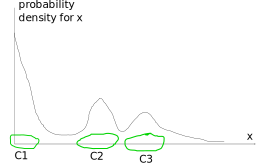
\includegraphics[width=0.5\textwidth]{cluster_illustration1.png}&\includegraphics[width=0.4\textwidth]{cluster_illustration2.png}\\ [-1.5ex]
  &{\fontsize{10}{0}\selectfont \textbf{Source: [MSD]}} \\
\end{tabular}
\newpage

%---------------------------------------------------------------
% PAGE EUCLIDEAN DISTANCE
% ----------------------------------------------------------------
\headerss{Euclidean distance}

\picngetwidth{0.25}{euclidean_distance.png}{\picwidth}
\parbox[b][0.25\textwidth][t]{0.95\textwidth - \picwidth}{
\begin{itemize}
\item In a two- or three-dimensional space this is simply a straight line between two points in the space
\item In the Cartesian co-ordinate system the distance can be calculated using Pythagoras' theorem
\item The distance between the points in the picture, A(2, 3) and B(7, 8), can be calculated as:

  {\scriptsize \vspace{-5ex}
    \begin{flalign}
    \nonumber d_{AB}&=\sqrt{(x_B - x_A)^2 + (y_B - y_A)^2}= \sqrt{(7-2)^2 + (8-3)^2} = \sqrt{50}= 7.07 && 
  \end{flalign}}
\end{itemize}
}

\sticktoprev
{\fontsize{10}{0}\selectfont \textbf{Source: [MSD]} \hfill}

\twoex\twoex
\xngetheight{\resizebox{\picwidth}{!}{\gendatatab}}{\gdtheight}
\parbox[b][\gdtheight][t]{0.95\textwidth - \picwidth}{
\begin{itemize}
\item In the general case, the Euclidean distance between data instances can be calculated for any number of dimensions representing attributes in the data set:
  
  {\scriptsize \vspace{-5ex}
    $$ d_{Ejk} = \sqrt{\sum_{i=1}^p (x_{ik}-x_{ij})^2} $$
  }
  where $x_1$, $x_2$... $x_p$ are numeric attributes and $d_{Ejk}$ is the Euclidean distance between instances $j$ and $k$.
\end{itemize}
}
\newpage

%---------------------------------------------------------------
% PAGE CATEGORICAL DATA DISTANCE
% ----------------------------------------------------------------
\headerss{Jaccard distance}

\begin{itemize}
\item The Jaccard distance is one example of how distance can be quantified between data instances based on categorical attribute values
\item In order for distances to be calculated, categorical data with more than two possible values is transformed into dichotomous data, by turning each value into a dichotomous attribute (for example, if a \textbf{colour} attribute had values \textbf{red}, \textbf{green} and \textbf{blue}, it would be transformed into three dichotomous attributes, each with possible values \textbf{0} or \textbf{1})
\end{itemize}

\xngetheight{\resizebox{\picwidth}{!}{\gendatatab}}{\dummy}
\parbox[b][\gdtheight - 1ex][t]{\textwidth - \picwidth}{
\begin{itemize}
\item Now, the Jaccard distance can be defined as:
  {\scriptsize 
    $$ d_{Jjk} = \dfrac{C_{01jk}+C_{10jk}}{C_{01jk}+C_{10jk}+C_{11jk}} $$
  }
where $C_{XYjk}$ is the number of attributes that have value $X$ in instance $j$ and value $Y$ in instance $k$ and $d_{Jjk}$ is the Jaccard distance between instances $j$ and $k$. $X$ and $Y$ are binary values (0 or 1).  
\end{itemize}}

\xngetheight{\resizebox{\picwidth}{!}{
\def\arraystretch{1.5}
\begin{tabular}{c c c c c c c} 
\hspace{3em} & $\pmb{x_1}$ & $\pmb{x_2}$ & $\pmb{x_3}$ & $\pmb{x_4}$ & $\pmb{x_5}$ & $\pmb{x_6}$ \\ 
\hline
$i_j$ & 0 & 1 & 0 & 1 & 0 & 1 \\
$i_k$ & 1 & 1 & 0 & 0 & 0 & 0 \\
\end{tabular}}}{\extabheight}
\parbox[b][\extabheight - 1ex][t]{\textwidth - \picwidth}{
  \begin{itemize}
  \item In the example shown on the left, the Jaccard distance is:
    {\scriptsize 
      $$d_{Jjk} = \dfrac{1+2}{1+2+1}= 0.75 $$
    }
  \end{itemize}
}
\newpage

%---------------------------------------------------------------
% PAGE HIERARCHICAL CLUSTERING
% ----------------------------------------------------------------
\headersec{Agglomerative hierarchical clustering}

\begin{itemize}
\item Agglomerative hierarchical clustering is an example of hierarchical clustering
\item It is a bottom up approach with the following high-level algorithm:
  \begin{enumerate}
  \item initially each instance in the data set is declared to be a cluster in itself (there are $n$ clusters, if $n$ is the number of data instances in the data set)
  \item the distance between each pair of clusters is calculated and the two clusters that are the closest are joined into a new cluster (the number of clusters is reduced by 1) 
  \item if the number of clusters is greater than 1, step 2 is repeated
  \end{enumerate}
  \textbf{Note:} Step 2 is performed $n-1$ times. An algorithm for distance to and from a cluster is used (lowest, highest or average).
\end{itemize}
\picngetwidth{0.19}{dendrogram.png}{\dendwidth}
\parbox[b][0.19\textwidth][t]{\textwidth - \dendwidth}{
    \begin{itemize}
      \item The number of clusters not set. Division into any number of clusters between $1$ and $n$ contained in result.
    \item The resultant tree can be shown as a \emph{dendrogram} (\emph{dendron}: \emph{tree} in Greek)
    \end{itemize}
  }
  
  \sticktoprev
  {\fontsize{10}{0}\selectfont \textbf{Source: [MSD]}}
\newpage

%---------------------------------------------------------------
% PAGE HIERARCHICAL CLUSTERING
% ----------------------------------------------------------------
\headersec{k-Means clustering}

\begin{itemize}
\item k-Means clustering is an example of non-hierarchical clustering
\item The algorithm is applied with prior knowledge of the number of clusters that should be created and can be described as follows:
  \begin{enumerate}
  \item the number of clusters, $k$, is set
  \item $k$ arbitrary points are chosen in the data-instance space (that defined by the data attributes) as initial \textbf{cluster representatives} $C_1$, $C_2$,...$C_k$
  \item for each instance in the data set, the closest cluster representative is determined and the instance assigned to cluster $j$, where $C_j$ is the closest cluster representative
    \item if no instance changes cluster (in 2\textsuperscript{nd} or subsequent iteration), the process is finished 
  \item if some instances moved to a new cluster, the cluster representatives are re-calculated so that each attribute gets the value average for that attribute among the data instances in the cluster (i.e. the centroid of the instances in the cluster becomes the cluster representative)
    \item repeat from step 3
  \end{enumerate}
\end{itemize}
\newpage

\headerss{Deciding on the optimal number of clusters}
\begin{itemize}
  
\item The optimal number of clusters is the highest number $k$ for which the $k$ clusters are significantly better in quality than the $k-1$ clusters arrived at using the same algorithm
  
\item Different measures are used for this but they are all based around the sum of within-cluster squares: $ S_{sawc} = \sum_{i=0}^n d_{iC(i)}^2 $, where $n$ is the number of instances in the set and $d_{iC(i)}$ is the distance between instance $i$ and the representative of the cluster it belongs to, $C(i)$
  
\end{itemize}
\picngetwidth{0.25}{elbow.png}{\elbowpngwidth}
\parbox[b][0.25\textwidth][t]{0.95\textwidth - \elbowpngwidth}{
\begin{itemize}
\item The value of the  within-cluster sum of squares is plotted against $k$ and the value of $k$ at which the negative slope becomes significantly less steep is the optimal value of $k$
\item Often the elbow-like shape, after which the method is named \emph{the elbow method}, is visually distinguishable in the graph
\item The method is not exact but does not need to be, since what is required is some indication of what value of $k$ provides a good balance between model complexity (in terms of the number of clusters) and model quality (in terms of the 'compactness' of the clusters)
\end{itemize}}

\sticktoprev{\fontsize{10}{0}\selectfont \textbf{Source: stackoverflow, user: Amro}}

\parbox[t]{\elbowpngwidth}{
\tiny \emph{The picture shows an elbow diagram for the well-known iris data set, containing data for 3 different types of iris. In  this case we know that 3 is the right number of clusters and the elbow diagram reflects this.}}


\newpage
  
%---------------------------------------------------------------
% PAGE ASSOCIATION RULES
% ----------------------------------------------------------------
\headerch{Association rules}
\hypertargettopofpage{assoc-rules}
\cornertab{N}{H}

\begin{itemize}
\item Association rules state the expectation of particular values of particular attributes ocurring together in a data instance
\item The following is an example of an association rule:

  \begin{tabular}{l}
    \texttt{IF customer is between 18 and 20 AND} \\
    \texttt{the customer buys a towel AND} \\
    \texttt{the customer buys a bath mat} \\
    \texttt{THEN the customer buys a shower curtain} \\
   \end{tabular}

 A small section of a data set for which that rule is defined, might look something like this: 

 \oneex
 \xngetheight{\resizebox{0.95\textwidth}{!}{
      \def\arraystretch{1.5}
      \begin{tabular}{|c c c c c c c c c c c c|} 
        \hline
        \textbf{TransactionId} & \textbf{Customer age} & $\hdots$ & \textbf{Towel} & \textbf{Bath mat} & \textbf{Shower curtain} & $\hdots$ & \textbf{Chewing gum} & $\hdots$ & \textbf{Milk} & \textbf{Biscuits} & $\hdots$ \\
        123456 & 20 & $\hdots$ & 1 & 1 & 1 & $\hdots$ & 1 & $\hdots$ & 0 & 0 & $\hdots$ \\
        123457 & 65 & $\hdots$ & 0 & 0 & 0 & $\hdots$ & 0 & $\hdots$ & 1 & 1 & $\hdots$ \\
        123458 & 26 & $\hdots$ & 0 & 0 & 0 & $\hdots$ & 1 & $\hdots$ & 1 & 0 & $\hdots$ \\
        \hline
      \end{tabular}}
    }{\artabheight}
    \oneex
    
    Each data instance (line in the table) represents a retail transaction in, let's say, a supermarket. The items sold in the shop are all represented with binary attributes, set to 0 if the item is absent from a transaction and to 1 if the item is present.
\newpage

%---------------------------- EXPLANATION-------------------------------------------
\item But, how are these rules arrived at? Some \textbf{measures} indicating levels of occurrence, co-ocurrence and likelihood of co-occurrence not being accidental are calculated for all the possible combinations of attributes, then the combinations with measure values indicative of association are stated in the form of association rules.

  Before we define the measures of interest, let us name the parts of an association rule:
  \begin{itemize}[label=\ding{213}]
  \item The \textbf{antecedent} is the condition in the rule i.e. the part between the IF and THEN. In the example, this is:

    \texttt{customer is between 18 and 20 AND the customer buys a towel AND the customer buys a bath mat}

  \item The \textbf{consequent} is the part that is true if the condition is fulfilled i.e. the part after THEN. In the example, this is:

    \texttt{the customer buys a shower curtain}
    
  \end{itemize}

  The most commonly used measures are:
  \begin{itemize}[label=\ding{51}]
    % ---------------------------- support -------------------------------------------
  \item \textbf{Support}: the probability of some combination of items occurring together. In particular, of interest is the \emph{support for the rule}, i.e. the probability of all the attribute values that appear in the rule occurring together in a data instance:

    \vspace{-2ex}
    {\small
      \begin{flalign}
        \nonumber &P(x_1 \in S_1 \wedge x_2 \in S_2 \wedge \hdots x_p \in S_p) &&
      \end{flalign}}
    
    \vspace{-2ex}
    where $P(A)$ is the probability of $A$, $x_1$, $x_2$ ... $x_p$ are the attributes of the data and $S_1$, $S_2$ ... $S_p$ are the sets of allowed values (one for each attribute) that define the combination of attribute values present in the rule. $\wedge$ is the logical AND operator. For the example, the support is:
    
    \vspace{-2ex}
    {\small
      \begin{flalign}
        \nonumber  P(customer\_age \in \{18, 19, 20\} &\wedge towel \in \{1\} \wedge bath\_mat \in \{1\} \wedge shower\_curtain \in \{1\}\ &&\\ 
        \nonumber &\wedge chewing\_gum \in \{0,1\} \wedge milk \in \{0,1\} \wedge biscuits \in \{0,1\})&&
      \end{flalign}}
    
    \vspace{-2ex}
    The expression includes all the attributes, but the ones that are not of interest are let have any value (e.g. \texttt{biscuits} could be there or not but we don't care, because we are looking for a relationship between \texttt{customer\_age}, presence of \texttt{towel}, presence of \texttt{bath\_mat} and presence of \texttt{shower\_curtain}, so \texttt{biscuits} is permitted any value i.e. 0 or 1). By leaving out the attributes that we don't care about and using more intuitive notation, the value for the support can be re-written as:
    
    \vspace{-2ex}
    {\small
      \begin{flalign}
        \nonumber &P((18 \leq customer\_age \leq 20) \wedge (towel = 1) \wedge (bath\_mat = 1) \wedge (shower\_curtain = 1)) &&
      \end{flalign}}
    
    \newpage
    
    % ---------------------------- confidence -------------------------------------------
  \item \textbf{Confidence}: the probability of the items in the combination occurring together, given the antecedent:
    
    \vspace{-2ex}
    {\small
      \begin{flalign}
        \nonumber &P(x_c \in S_c  \, \mathlarger{|} \, x_1 \in S_1 \wedge x_2 \in S_2 \wedge \hdots \boldsymbol{x_{c-1} \in S_{c-1} \wedge x_{c+1} \in S_{c+1}} \wedge \hdots x_p \in S_p)=  &&
      \end{flalign}}
    \vspace{-1ex}
    {\small
      \begin{flalign}
        \nonumber &\dfrac{P(x_1 \in S_1 \wedge x_2 \in S_2 \wedge \hdots  x_p \in S_p)}{P(x_1 \in S_1 \wedge x_2 \in S_2 \wedge \hdots \boldsymbol{x_{c-1} \in S_{c-1} \wedge x_{c+1} \in S_{c+1}} \wedge \hdots x_p \in S_p)}  && 
      \end{flalign}}
    
    \vspace{-2ex}
    where $P(A|B)$ is the probability of $A$, given $B$, $x_1$, $x_2$ ... $x_p$ are the attributes of the data and $S_1$, $S_2$ ... $S_p$ are the sets of allowed values (one for each attribute) that define the combination of attribute values present in the rule. The attribute $x_c$ represents the attribute that features in the \emph{consequent} of the rule and $S_c$ is the set of values that the consequent allows for this attribute (the consequent could feature more than one attribute but we will only look at the case where one attribute is involved). It is absent from the combination of attribute values that define the \emph{antecedent} (the part of the attribute list from which $x_c$ is missing is shown in boldface). The confidence is calculated by dividing the support for the entire rule by the support for the antecedent (the part of the equation after the equal sign).
    
    The confidence for the example is:
    {\small
      \begin{flalign}
        \nonumber &P(shower\_curtain=1 \, \mathlarger{|} \, (18 \leq customer\_age \leq 20) \wedge (towel = 1) \wedge (bath\_mat = 1)) &&
      \end{flalign}}

  %--------------------------------------- lift --------------------------------------------
  \item \textbf{Lift}: the ratio between the actual probability of the items in the combination occurring together and the the probability of the co-occurrence happening by chance  :
    
    \vspace{-2ex}
    {\small
      \begin{flalign}
        \nonumber &\dfrac{P(x_1 \in S_1 \wedge x_2 \in S_2 \wedge \hdots  x_p \in S_p)}{P(x_1 \in S_1 \wedge x_2 \in S_2 \wedge \hdots \boldsymbol{x_{c-1} \in S_{c-1} \wedge x_{c+1} \in S_{c+1}} \wedge \hdots x_p \in S_p)P(x_c \in S_c)}  && 
      \end{flalign}}
    
    \vspace{-2ex}
    Three probabilities feature in the formula, each the \emph{support} for different part of the rule:
    \begin{itemize}
    \item the entire rule:
      {\small $P(x_1 \in S_1 \wedge x_2 \in S_2 \wedge \hdots  x_p \in S_p)$ }
    \item the antecedent:
      {\small $P(x_1 \in S_1 \wedge x_2 \in S_2 \wedge \hdots \boldsymbol{x_{c-1} \in S_{c-1} \wedge x_{c+1} \in S_{c+1}} \wedge \hdots x_p \in S_p)$}
    \item the consequent:
      {\small $P(x_c \in S_c)$}
    \end{itemize}
    
    The lift for the example is:
    {\small
      \begin{flalign}
        \nonumber &\dfrac{P((18 \leq customer\_age \leq 20) \wedge (towel = 1) \wedge (bath\_mat = 1) \wedge (shower\_curtain=1))}{P((18 \leq customer\_age \leq 20) \wedge (towel = 1) \wedge (bath\_mat = 1))P(shower\_curtain=1)} &&
      \end{flalign}}
  \end{itemize}

\item Association rules are mined from the data by setting required levels for the different measures, for example $50\%$ rule support, $50\%$ confidence and a lift of $3$, then searching for rules that meet these minimal requirements.
\item The \textbf{apriori} method is based around the fact that support for a value combination is always the same or lower than that of any of its subset combinations. It starts with a search for single-value combinations that meet the support level, progressing onto 2-value combinations that are supersets of the retained 1-value combinations and so on.
\end{itemize}

\twoex
  \picngetwidth{0.25}{association_rules_example.png}{\assocruleexwidth}
  \parbox[b][0.25\textwidth][t]{0.95\textwidth - \assocruleexwidth}{\tiny \emph{A rule for this data set and associated measures are as follows:}

   \oneex
    \begin{tabular}{l}
      \emph{\texttt{IF \textbf{colour} = gray AND}}  \\
      \emph{\texttt{\textbf{shape} = circle}} \\
      \emph{\texttt{THEN \textbf{border} = thick}} \\
    \end{tabular}

    \oneex
    \begin{itemize}
    \item \emph{\textbf{support}: 6/26 (there are 6 out of 26 elements have the three values included in the definition of the rule: \texttt{B, E, G, K, M, P})}
    \item \emph{\textbf{confidence}: 6/7 (we divide the support for the rule 6/26 with the support for the antecedent, which is 7/26, as the antecedent is true for element \texttt{W} in addition to those that support the entire rule)}
    \item \emph{\textbf{lift}: $\dfrac{6/26}{(7/26)\times(14/26)} = 1.59 $}

      \emph{The lift value means that the antecedent and consequent occur together 1.59 times more often than they would by pure chance.}
    \end{itemize}}

\sticktoprev
{\fontsize{10}{0}\selectfont \textbf{Source: [MSD]} \hfill}

\vspace{-1ex}
\parbox[t]{\assocruleexwidth}{\tiny \emph{The picture shows a set of elements with three attributes: \texttt{\textbf{shape}}, \texttt{\textbf{color}} and \texttt{\textbf{border}} with respective value sets \texttt{\{circle, square\}}, \texttt{\{white, gray\}} and \texttt{\{thin, thick\}}. The elements represent data instances.}}



\newpage

%----------------------------------------------------------------
% PAGE REFERENCES
% ----------------------------------------------------------------
\headersec{References}

The pictures in this presentation were taken from the following books. The source for each picture is cited beside it. 

\textbf{[MSD]} \emph{Making Sense of Data I: A Practical Guide to Exploratory Data Analysis and Data Mining}, by Glenn J. Myatt and Wayne P. Johnson, John Wiley \& Sons, 2014. 









\end{document}
